% Generated by Sphinx.
\def\sphinxdocclass{report}
\documentclass[letterpaper,10pt,english]{sphinxmanual}
\usepackage[utf8]{inputenc}
\DeclareUnicodeCharacter{00A0}{\nobreakspace}
\usepackage{cmap}
\usepackage[T1]{fontenc}
\usepackage{babel}
\usepackage{times}
\usepackage[Bjarne]{fncychap}
\usepackage{longtable}
\usepackage{sphinx}
\usepackage{multirow}

\addto\captionsenglish{\renewcommand{\figurename}{Fig. }}
\addto\captionsenglish{\renewcommand{\tablename}{Table }}
\floatname{literal-block}{Listing }

\usepackage{amsfonts,amsmath}

\title{CySparse's developers manual}
\date{December 23, 2015}
\release{0.2.2}
\author{Nikolaj van Omme\\Sylvain Arreckx\\Dominique Orban}
\newcommand{\sphinxlogo}{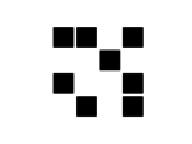
\includegraphics{cysparse_logo128.pdf}\par}
\renewcommand{\releasename}{Release}
\makeindex

\makeatletter
\def\PYG@reset{\let\PYG@it=\relax \let\PYG@bf=\relax%
    \let\PYG@ul=\relax \let\PYG@tc=\relax%
    \let\PYG@bc=\relax \let\PYG@ff=\relax}
\def\PYG@tok#1{\csname PYG@tok@#1\endcsname}
\def\PYG@toks#1+{\ifx\relax#1\empty\else%
    \PYG@tok{#1}\expandafter\PYG@toks\fi}
\def\PYG@do#1{\PYG@bc{\PYG@tc{\PYG@ul{%
    \PYG@it{\PYG@bf{\PYG@ff{#1}}}}}}}
\def\PYG#1#2{\PYG@reset\PYG@toks#1+\relax+\PYG@do{#2}}

\expandafter\def\csname PYG@tok@gd\endcsname{\def\PYG@tc##1{\textcolor[rgb]{0.63,0.00,0.00}{##1}}}
\expandafter\def\csname PYG@tok@gu\endcsname{\let\PYG@bf=\textbf\def\PYG@tc##1{\textcolor[rgb]{0.50,0.00,0.50}{##1}}}
\expandafter\def\csname PYG@tok@gt\endcsname{\def\PYG@tc##1{\textcolor[rgb]{0.00,0.27,0.87}{##1}}}
\expandafter\def\csname PYG@tok@gs\endcsname{\let\PYG@bf=\textbf}
\expandafter\def\csname PYG@tok@gr\endcsname{\def\PYG@tc##1{\textcolor[rgb]{1.00,0.00,0.00}{##1}}}
\expandafter\def\csname PYG@tok@cm\endcsname{\let\PYG@it=\textit\def\PYG@tc##1{\textcolor[rgb]{0.25,0.50,0.56}{##1}}}
\expandafter\def\csname PYG@tok@vg\endcsname{\def\PYG@tc##1{\textcolor[rgb]{0.73,0.38,0.84}{##1}}}
\expandafter\def\csname PYG@tok@m\endcsname{\def\PYG@tc##1{\textcolor[rgb]{0.13,0.50,0.31}{##1}}}
\expandafter\def\csname PYG@tok@mh\endcsname{\def\PYG@tc##1{\textcolor[rgb]{0.13,0.50,0.31}{##1}}}
\expandafter\def\csname PYG@tok@cs\endcsname{\def\PYG@tc##1{\textcolor[rgb]{0.25,0.50,0.56}{##1}}\def\PYG@bc##1{\setlength{\fboxsep}{0pt}\colorbox[rgb]{1.00,0.94,0.94}{\strut ##1}}}
\expandafter\def\csname PYG@tok@ge\endcsname{\let\PYG@it=\textit}
\expandafter\def\csname PYG@tok@vc\endcsname{\def\PYG@tc##1{\textcolor[rgb]{0.73,0.38,0.84}{##1}}}
\expandafter\def\csname PYG@tok@il\endcsname{\def\PYG@tc##1{\textcolor[rgb]{0.13,0.50,0.31}{##1}}}
\expandafter\def\csname PYG@tok@go\endcsname{\def\PYG@tc##1{\textcolor[rgb]{0.20,0.20,0.20}{##1}}}
\expandafter\def\csname PYG@tok@cp\endcsname{\def\PYG@tc##1{\textcolor[rgb]{0.00,0.44,0.13}{##1}}}
\expandafter\def\csname PYG@tok@gi\endcsname{\def\PYG@tc##1{\textcolor[rgb]{0.00,0.63,0.00}{##1}}}
\expandafter\def\csname PYG@tok@gh\endcsname{\let\PYG@bf=\textbf\def\PYG@tc##1{\textcolor[rgb]{0.00,0.00,0.50}{##1}}}
\expandafter\def\csname PYG@tok@ni\endcsname{\let\PYG@bf=\textbf\def\PYG@tc##1{\textcolor[rgb]{0.84,0.33,0.22}{##1}}}
\expandafter\def\csname PYG@tok@nl\endcsname{\let\PYG@bf=\textbf\def\PYG@tc##1{\textcolor[rgb]{0.00,0.13,0.44}{##1}}}
\expandafter\def\csname PYG@tok@nn\endcsname{\let\PYG@bf=\textbf\def\PYG@tc##1{\textcolor[rgb]{0.05,0.52,0.71}{##1}}}
\expandafter\def\csname PYG@tok@no\endcsname{\def\PYG@tc##1{\textcolor[rgb]{0.38,0.68,0.84}{##1}}}
\expandafter\def\csname PYG@tok@na\endcsname{\def\PYG@tc##1{\textcolor[rgb]{0.25,0.44,0.63}{##1}}}
\expandafter\def\csname PYG@tok@nb\endcsname{\def\PYG@tc##1{\textcolor[rgb]{0.00,0.44,0.13}{##1}}}
\expandafter\def\csname PYG@tok@nc\endcsname{\let\PYG@bf=\textbf\def\PYG@tc##1{\textcolor[rgb]{0.05,0.52,0.71}{##1}}}
\expandafter\def\csname PYG@tok@nd\endcsname{\let\PYG@bf=\textbf\def\PYG@tc##1{\textcolor[rgb]{0.33,0.33,0.33}{##1}}}
\expandafter\def\csname PYG@tok@ne\endcsname{\def\PYG@tc##1{\textcolor[rgb]{0.00,0.44,0.13}{##1}}}
\expandafter\def\csname PYG@tok@nf\endcsname{\def\PYG@tc##1{\textcolor[rgb]{0.02,0.16,0.49}{##1}}}
\expandafter\def\csname PYG@tok@si\endcsname{\let\PYG@it=\textit\def\PYG@tc##1{\textcolor[rgb]{0.44,0.63,0.82}{##1}}}
\expandafter\def\csname PYG@tok@s2\endcsname{\def\PYG@tc##1{\textcolor[rgb]{0.25,0.44,0.63}{##1}}}
\expandafter\def\csname PYG@tok@vi\endcsname{\def\PYG@tc##1{\textcolor[rgb]{0.73,0.38,0.84}{##1}}}
\expandafter\def\csname PYG@tok@nt\endcsname{\let\PYG@bf=\textbf\def\PYG@tc##1{\textcolor[rgb]{0.02,0.16,0.45}{##1}}}
\expandafter\def\csname PYG@tok@nv\endcsname{\def\PYG@tc##1{\textcolor[rgb]{0.73,0.38,0.84}{##1}}}
\expandafter\def\csname PYG@tok@s1\endcsname{\def\PYG@tc##1{\textcolor[rgb]{0.25,0.44,0.63}{##1}}}
\expandafter\def\csname PYG@tok@gp\endcsname{\let\PYG@bf=\textbf\def\PYG@tc##1{\textcolor[rgb]{0.78,0.36,0.04}{##1}}}
\expandafter\def\csname PYG@tok@sh\endcsname{\def\PYG@tc##1{\textcolor[rgb]{0.25,0.44,0.63}{##1}}}
\expandafter\def\csname PYG@tok@ow\endcsname{\let\PYG@bf=\textbf\def\PYG@tc##1{\textcolor[rgb]{0.00,0.44,0.13}{##1}}}
\expandafter\def\csname PYG@tok@sx\endcsname{\def\PYG@tc##1{\textcolor[rgb]{0.78,0.36,0.04}{##1}}}
\expandafter\def\csname PYG@tok@bp\endcsname{\def\PYG@tc##1{\textcolor[rgb]{0.00,0.44,0.13}{##1}}}
\expandafter\def\csname PYG@tok@c1\endcsname{\let\PYG@it=\textit\def\PYG@tc##1{\textcolor[rgb]{0.25,0.50,0.56}{##1}}}
\expandafter\def\csname PYG@tok@kc\endcsname{\let\PYG@bf=\textbf\def\PYG@tc##1{\textcolor[rgb]{0.00,0.44,0.13}{##1}}}
\expandafter\def\csname PYG@tok@c\endcsname{\let\PYG@it=\textit\def\PYG@tc##1{\textcolor[rgb]{0.25,0.50,0.56}{##1}}}
\expandafter\def\csname PYG@tok@mf\endcsname{\def\PYG@tc##1{\textcolor[rgb]{0.13,0.50,0.31}{##1}}}
\expandafter\def\csname PYG@tok@err\endcsname{\def\PYG@bc##1{\setlength{\fboxsep}{0pt}\fcolorbox[rgb]{1.00,0.00,0.00}{1,1,1}{\strut ##1}}}
\expandafter\def\csname PYG@tok@mb\endcsname{\def\PYG@tc##1{\textcolor[rgb]{0.13,0.50,0.31}{##1}}}
\expandafter\def\csname PYG@tok@ss\endcsname{\def\PYG@tc##1{\textcolor[rgb]{0.32,0.47,0.09}{##1}}}
\expandafter\def\csname PYG@tok@sr\endcsname{\def\PYG@tc##1{\textcolor[rgb]{0.14,0.33,0.53}{##1}}}
\expandafter\def\csname PYG@tok@mo\endcsname{\def\PYG@tc##1{\textcolor[rgb]{0.13,0.50,0.31}{##1}}}
\expandafter\def\csname PYG@tok@kd\endcsname{\let\PYG@bf=\textbf\def\PYG@tc##1{\textcolor[rgb]{0.00,0.44,0.13}{##1}}}
\expandafter\def\csname PYG@tok@mi\endcsname{\def\PYG@tc##1{\textcolor[rgb]{0.13,0.50,0.31}{##1}}}
\expandafter\def\csname PYG@tok@kn\endcsname{\let\PYG@bf=\textbf\def\PYG@tc##1{\textcolor[rgb]{0.00,0.44,0.13}{##1}}}
\expandafter\def\csname PYG@tok@o\endcsname{\def\PYG@tc##1{\textcolor[rgb]{0.40,0.40,0.40}{##1}}}
\expandafter\def\csname PYG@tok@kr\endcsname{\let\PYG@bf=\textbf\def\PYG@tc##1{\textcolor[rgb]{0.00,0.44,0.13}{##1}}}
\expandafter\def\csname PYG@tok@s\endcsname{\def\PYG@tc##1{\textcolor[rgb]{0.25,0.44,0.63}{##1}}}
\expandafter\def\csname PYG@tok@kp\endcsname{\def\PYG@tc##1{\textcolor[rgb]{0.00,0.44,0.13}{##1}}}
\expandafter\def\csname PYG@tok@w\endcsname{\def\PYG@tc##1{\textcolor[rgb]{0.73,0.73,0.73}{##1}}}
\expandafter\def\csname PYG@tok@kt\endcsname{\def\PYG@tc##1{\textcolor[rgb]{0.56,0.13,0.00}{##1}}}
\expandafter\def\csname PYG@tok@sc\endcsname{\def\PYG@tc##1{\textcolor[rgb]{0.25,0.44,0.63}{##1}}}
\expandafter\def\csname PYG@tok@sb\endcsname{\def\PYG@tc##1{\textcolor[rgb]{0.25,0.44,0.63}{##1}}}
\expandafter\def\csname PYG@tok@k\endcsname{\let\PYG@bf=\textbf\def\PYG@tc##1{\textcolor[rgb]{0.00,0.44,0.13}{##1}}}
\expandafter\def\csname PYG@tok@se\endcsname{\let\PYG@bf=\textbf\def\PYG@tc##1{\textcolor[rgb]{0.25,0.44,0.63}{##1}}}
\expandafter\def\csname PYG@tok@sd\endcsname{\let\PYG@it=\textit\def\PYG@tc##1{\textcolor[rgb]{0.25,0.44,0.63}{##1}}}

\def\PYGZbs{\char`\\}
\def\PYGZus{\char`\_}
\def\PYGZob{\char`\{}
\def\PYGZcb{\char`\}}
\def\PYGZca{\char`\^}
\def\PYGZam{\char`\&}
\def\PYGZlt{\char`\<}
\def\PYGZgt{\char`\>}
\def\PYGZsh{\char`\#}
\def\PYGZpc{\char`\%}
\def\PYGZdl{\char`\$}
\def\PYGZhy{\char`\-}
\def\PYGZsq{\char`\'}
\def\PYGZdq{\char`\"}
\def\PYGZti{\char`\~}
% for compatibility with earlier versions
\def\PYGZat{@}
\def\PYGZlb{[}
\def\PYGZrb{]}
\makeatother

\renewcommand\PYGZsq{\textquotesingle}

\begin{document}

\maketitle
\tableofcontents
\phantomsection\label{contents::doc}

\begin{quote}\begin{description}
\item[{Release}] \leavevmode
0.2

\item[{Date}] \leavevmode
December 23, 2015

\end{description}\end{quote}


\chapter{Introduction}
\label{introduction:introduction}\label{introduction::doc}\label{introduction:cysparse-s-developers-manual}
Welcome to \textbf{\texttt{CySparse}}`s developers manual!

\textbf{\texttt{CySparse}} is a fast sparse matrix library for \textbf{\texttt{Python}}/\textbf{\texttt{Cython}}.

\begin{notice}{warning}{Warning:}
This is the manual for \textbf{developers}.
\end{notice}

Maintening a library as \textbf{\texttt{CySparse}} is not a small task. This is partly due to:
\begin{itemize}
\item {} 
the mix of several programming languages (mainly \textbf{\texttt{Cython}}, \textbf{\texttt{Python}} and \textbf{\texttt{C}});

\item {} 
the use of templated source files;

\item {} 
the use of several external tools (\href{https://github.com/PythonOptimizers/cygenja}{cygenja}, \href{http://jinja.pocoo.org/}{Jinja2}, \href{http://sphinx-doc.org/}{Sphinx}, \href{https://www.latex-project.org/}{LaTeX}, etc.);

\item {} 
the optimized code (several code chuncks are highly optimized for speed);

\item {} 
the coupling with \href{http://www.numpy.org/}{NumPy};

\item {} 
the language \href{http://cython.org/}{Cython} that is not really mature yet. The team behind \textbf{\texttt{Cython}} is doing a fantastic job but the language still has numerous bugs. If you've never used a compiler with bugs, welcome to this wonderful world were you might have
to debug the compiler as much as your code (yep!);

\end{itemize}


\chapter{Sparse Matrix Formats}
\label{sparse_matrix_formats:sparse-matrix-formats}\label{sparse_matrix_formats::doc}\label{sparse_matrix_formats:id1}
{[}THIS SECTION IS VERY DETAILED AND IS PROBABLY NOT INTENDED FOR THE COMMON USER{]}

This section describes the sparse matrix storage schemes available in
\textbf{\texttt{Cysparse}}. In the next sections, we cover sparse matrix creation, population, view and conversion.

Basically, we use one general sparse matrix format to \emph{create} a general sparse matrix: the \code{LLSparseMatrix} class. This class has
a rich API and allows multiple ways to create and transform a sparse matrix. Once the matrix is ready to be used, it can be appropriately converted
into a specialized sparse matrix format that is optimized for the needed operations. The \code{LLSparseMatrix} is also the only type of matrices that
can be modified while the other types of matrices are \textbf{immutable} for efficiency.

Here is a list of existing formats and their basic use:
\begin{itemize}
\item {} 
Linked-list format (\code{LL}): a convenient format for creating and populating
a sparse matrix, whether symmetric or general.

\item {} 
Compressed sparse row format (\code{CSR}): a format designed to speed up
matrix-vector products.

\item {} 
Compressed sparse column format (\code{CSC}): a format designed to speed up
vector-matrix products.

\end{itemize}

The CSR and CSC formats are complementary and can be viewed as respectively a row- and column view of a sparse matrix.

These formats are well known in the community and you can find scores of documents about them on the internet.


\section{Sorted column and row indices}
\label{sparse_matrix_formats:sorted-column-and-row-indices}
{[}TO BE WRITTEN{]}

For all sparse matrix formats, we internally keep the indices sorted, i.e. in ascending order.


\section{The \texttt{LL} sparse format in details}
\label{sparse_matrix_formats:the-ll-sparse-format-in-details}
This format is implemented by the \code{LLSparseMatrix} class.

All matrix classes are straightforward with perhaps the only exception of the \code{LLSparseMatrix} class. This class is really a container where you can easily add or remove elements but it is not much more than that: a container. As such, it is \textbf{not} optimized for any matrix operation. There are some internal optimisations though to add or retrieve an element and we explain them here.


\subsection{Elements are linked in chains (aka linked lists)}
\label{sparse_matrix_formats:elements-are-linked-in-chains-aka-linked-lists}
The \code{LLSparseMatrix} container is made of 4 one dimensionnal arrays and one pointer (\code{free}):
\begin{itemize}
\item {} 
\code{root{[}i{]}}: points to the first elements of row \code{i};

\item {} 
\code{col{[}k{]}}: contains the column index \code{j} of an element stored at the \code{k}-th place;

\item {} 
\code{val{[}k{]}}: contains the value of the element stored at the \code{k}-th place;

\item {} 
\code{link{[}k{]}}: contains the pointer to the next element in the chain where the \code{k}-th element belongs.

\end{itemize}

The pointer \code{free} points to the first free element in the chain of free elements.

Despite its name, \emph{linked list} sparse matrix, this container doesn't use list of pointers but \textbf{only} arrays of indices. ``Pointers'' are indices in arrays and to denote a pointer to \code{NULL} the value \code{-1} if used. For instance, if \code{free == -1},
this means that the chain of free elements is empty.

Then chain can be traversed by following the \code{link} array:
\begin{figure}[htbp]
\centering
\capstart

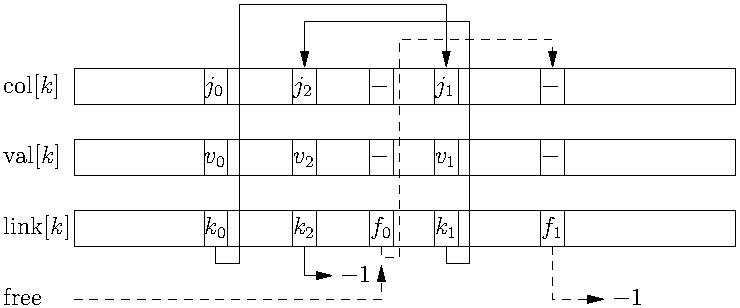
\includegraphics[width=400pt]{ll_mat_link.pdf}
\caption{Chains in an \code{LLSparseMatrix} matrix}\end{figure}

Two chains are depicted in the picture. First, the chain with free elements. These are elements that where removed. The \code{free} pointer points to the first element of this chain and \code{link{[}free{]}} if \(f_0\) which points to
the second element in this chain. Whenever a new elements is added, it will take the place of this first element.

The second chain starts with element (\(j_0\), \(v_0\), \(k_0\)). \(k_0\) points to the second element (\(j_1\), \(v_1\), \(k_1\)) and \(k_1\) points to the second and last element (\(j_2\), \(v_2\), \(k_2\)).

Inside the arrays, the elements can be stored in any order.


\subsection{Elements are ``aligned'' row wise (chains correspond to rows)}
\label{sparse_matrix_formats:elements-are-aligned-row-wise-chains-correspond-to-rows}
Each chain of elements corresponds to one row of the matrix. The pointer \code{root{[}i{]}} points to the first element of the \code{i} $^{\text{th}}$ row. If the above chain (\(k_0\), \(k_1\) and \(k_2\) ) correspond to the only
elements on row \code{i}, \code{root{[}i{]}} would point to element (\(j_0\), \(v_0\), \(k_0\)). If row \code{i} doesn't have any element, \code{root{[}i{]} == -1}.

To traverse the \code{i}$^{\text{th}}$ row, simply use:

\begin{Verbatim}[commandchars=\\\{\}]
\PYG{n}{k} \PYG{o}{=} \PYG{n+nb+bp}{self}\PYG{o}{.}\PYG{n}{root}\PYG{p}{[}\PYG{n}{i}\PYG{p}{]}

\PYG{k}{while} \PYG{n}{k} \PYG{o}{!=} \PYG{o}{\PYGZhy{}}\PYG{l+m+mi}{1}\PYG{p}{:}
    \PYG{c}{\PYGZsh{} we consider element A[i, j] == val}
    \PYG{n}{j} \PYG{o}{=} \PYG{n+nb+bp}{self}\PYG{o}{.}\PYG{n}{col}\PYG{p}{[}\PYG{n}{k}\PYG{p}{]}
    \PYG{n}{val} \PYG{o}{=} \PYG{n+nb+bp}{self}\PYG{o}{.}\PYG{n}{val}\PYG{p}{[}\PYG{n}{k}\PYG{p}{]}
    \PYG{o}{.}\PYG{o}{.}\PYG{o}{.}
    \PYG{n}{k} \PYG{o}{=} \PYG{n+nb+bp}{self}\PYG{o}{.}\PYG{n}{link}\PYG{p}{[}\PYG{n}{k}\PYG{p}{]}
\end{Verbatim}


\subsection{Inside a row, elements are ordered by column order (how to run through a \texttt{LL} matrix)}
\label{sparse_matrix_formats:inside-a-row-elements-are-ordered-by-column-order-how-to-run-through-a-ll-matrix}
If the chain corresponding to row \code{i} is \(k_0, k_1, \ldots, k_p\), then we know that the corresponding column indices are ordered: \(j_0 < j_1 < \ldots < j_p\). When an element is added with the \code{put(i, j, val)} method, this new element is inserted in the right place, swapping pointers elements of \code{link} if necessary.

This means that looking for an element \code{A{[}i, k{]}}, one can simply use:

\begin{Verbatim}[commandchars=\\\{\}]
\PYG{n}{k} \PYG{o}{=} \PYG{n+nb+bp}{self}\PYG{o}{.}\PYG{n}{root}\PYG{p}{[}\PYG{n}{i}\PYG{p}{]}

\PYG{k}{while} \PYG{n}{k} \PYG{o}{!=} \PYG{o}{\PYGZhy{}}\PYG{l+m+mi}{1}\PYG{p}{:}

    \PYG{k}{if} \PYG{n+nb+bp}{self}\PYG{o}{.}\PYG{n}{col}\PYG{p}{[}\PYG{n}{k}\PYG{p}{]} \PYG{o}{\PYGZgt{}} \PYG{n}{j}\PYG{p}{:}
        \PYG{c}{\PYGZsh{} element doesn\PYGZsq{}t exist}
        \PYG{k}{break}

    \PYG{k}{if} \PYG{n+nb+bp}{self}\PYG{o}{.}\PYG{n}{col}\PYG{p}{[}\PYG{n}{k}\PYG{p}{]} \PYG{o}{==} \PYG{n}{j}\PYG{p}{:}
        \PYG{c}{\PYGZsh{} element exists}
        \PYG{o}{.}\PYG{o}{.}\PYG{o}{.}

    \PYG{n}{k} \PYG{o}{=} \PYG{n+nb+bp}{self}\PYG{o}{.}\PYG{n}{link}\PYG{p}{[}\PYG{n}{k}\PYG{p}{]}
\end{Verbatim}


\subsection{Insertion of a new element in more details}
\label{sparse_matrix_formats:insertion-of-a-new-element-in-more-details}
The next figure represent the internal state of a \code{LLSparseMatrix}:
\begin{figure}[htbp]
\centering
\capstart

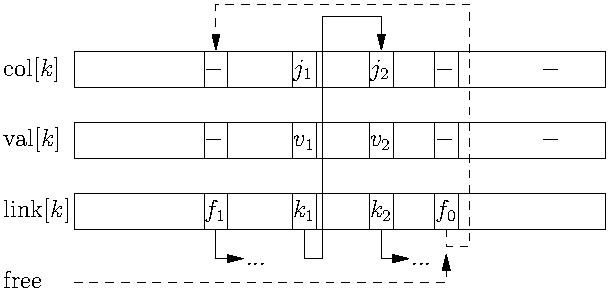
\includegraphics[width=300pt]{ll_mat_link_swap_left.pdf}
\caption{\textbf{Before} insertion of element \((j, v, k)\) in a \code{LLSparseMatrix} matrix}\end{figure}

We have \(j_1 < j_2\) and \(k_1\) points to element \(k_2\). Let's say we want to insert an new element \((j, v, k)\) with column index \(j\) such that \(j_1 <  j < j_2\).
To preserve the ordering, we have to insert this element \textbf{between} the elements \(k_1\) and \(k_2\) as shown on the following figure:
\begin{figure}[htbp]
\centering
\capstart

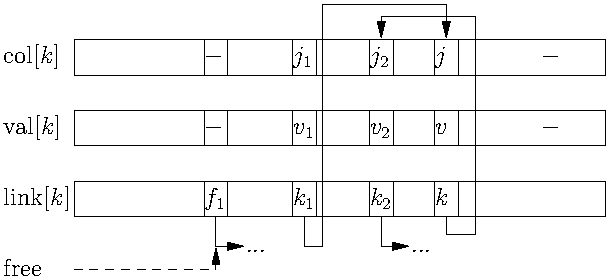
\includegraphics[width=300pt]{ll_mat_link_swap_right.pdf}
\caption{\textbf{After} insertion of element \((j, v, k)\) in a \code{LLSparseMatrix} matrix}\end{figure}

The element \((j, v, k)\) was inserted in place of the first free element pointed by \code{free} and \(k_1\) now points to this element. Notice also that now, \code{free} points to the next free element \(f_1\).


\subsection{Detailed example}
\label{sparse_matrix_formats:detailed-example}
For all sparse matrix formats, we'll detail an example. Let \(A\) be the following \(3 \times 4\) sparse matrix:
\begin{figure}[htbp]
\centering
\capstart

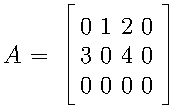
\includegraphics[width=100pt]{detailed_example_smatrix_formats.pdf}
\caption{The example sparse matrix \(A\)}\end{figure}

Notice that this matrix is sparse with 4 non zero entries, is non symmetric and has an empty row and column.


\subsection{How to run through a \texttt{LL} matrix}
\label{sparse_matrix_formats:how-to-run-through-a-ll-matrix}
To find all triplets \((i, j, v)\):

\begin{Verbatim}[commandchars=\\\{\}]
\PYG{k}{for} \PYG{n}{i} \PYG{k+kn}{from} \PYG{l+m+mi}{0} \PYG{o}{\PYGZlt{}}\PYG{o}{=} \PYG{n}{i} \PYG{o}{\PYGZlt{}} \PYG{n}{nrow}\PYG{p}{:}
    \PYG{n}{k} \PYG{o}{=} \PYG{n+nb+bp}{self}\PYG{o}{.}\PYG{n}{root}\PYG{p}{[}\PYG{n}{i}\PYG{p}{]}
    \PYG{k}{while} \PYG{n}{k} \PYG{o}{!=} \PYG{o}{\PYGZhy{}}\PYG{l+m+mi}{1}\PYG{p}{:}
       \PYG{n}{j} \PYG{o}{=} \PYG{n+nb+bp}{self}\PYG{o}{.}\PYG{n}{col}\PYG{p}{[}\PYG{n}{k}\PYG{p}{]}
       \PYG{n}{v} \PYG{o}{=} \PYG{n+nb+bp}{self}\PYG{o}{.}\PYG{n}{val}\PYG{p}{[}\PYG{n}{k}\PYG{p}{]}

       \PYG{n}{k} \PYG{o}{=} \PYG{n+nb+bp}{self}\PYG{o}{.}\PYG{n}{link}\PYG{p}{[}\PYG{n}{k}\PYG{p}{]}
\end{Verbatim}


\section{The \texttt{CSR} sparse format in details}
\label{sparse_matrix_formats:the-csr-sparse-format-in-details}
This format is implemented by the \code{CSRSparseMatrix} class. This format use a row-wise representation, as the above \code{LL} Sparse format, i.e. elements are stored row by row.


\subsection{Detailed example}
\label{sparse_matrix_formats:id2}
Here are the three internal arrays for the example matrix:
\begin{figure}[htbp]
\centering
\capstart

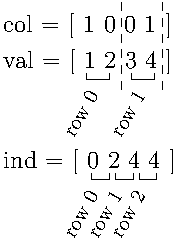
\includegraphics[width=100pt]{csr_detailed_example.pdf}
\caption{The internal arrays of a \code{CSR} matrix}\end{figure}

One can immediatly see that the values are stored row-wise in \code{col} and \code{val}: first the row \code{0}, than the row \code{1} (and nothing for row \code{2}). \code{ind} gives the first indices for each row: \code{ind{[}0{]} == 0} gives the start of row \code{0},
\code{ind{[}1{]} == 2} gives the start of row \code{1}, etc. This means that \code{ind{[}i+1{]} - ind{[}i{]}} returns the number of elements in row \code{i}.


\subsection{How to run through a \texttt{CSR} matrix}
\label{sparse_matrix_formats:how-to-run-through-a-csr-matrix}
To find all triplets \((i, j, v)\):

\begin{Verbatim}[commandchars=\\\{\}]
\PYG{k}{for} \PYG{n}{i} \PYG{k+kn}{from} \PYG{l+m+mi}{0} \PYG{o}{\PYGZlt{}}\PYG{o}{=} \PYG{n}{i} \PYG{o}{\PYGZlt{}} \PYG{n}{nrow}\PYG{p}{:}
    \PYG{k}{for} \PYG{n}{k} \PYG{k+kn}{from} \PYG{n+nn}{ind}\PYG{p}{[}\PYG{n}{i}\PYG{p}{]} \PYG{o}{\PYGZlt{}}\PYG{o}{=} \PYG{n}{k} \PYG{o}{\PYGZlt{}} \PYG{n}{ind}\PYG{p}{[}\PYG{n}{i}\PYG{o}{+}\PYG{l+m+mi}{1}\PYG{p}{]}\PYG{p}{:}
        \PYG{n}{j} \PYG{o}{=} \PYG{n}{col}\PYG{p}{[}\PYG{n}{k}\PYG{p}{]}
        \PYG{n}{v} \PYG{o}{=} \PYG{n}{val}\PYG{p}{[}\PYG{n}{k}\PYG{p}{]}
\end{Verbatim}


\section{The \texttt{CSC} sparse format in details}
\label{sparse_matrix_formats:the-csc-sparse-format-in-details}
This format is implemented by the \code{CSCSparseMatrix} class.

The \code{CSC} sparse matrix format is exactly the same as the CSR sparse matrix format but column-wise. Given a matrix \(A\) and a \code{CSR} representation of this matrix is exactly the same as a \code{CSC} respresentation
of the transposed matrix \(A^t\), i.e.
\begin{gather}
\begin{split}\textrm{CSR}(A) = \textrm{CSC}(A^t)\end{split}\notag
\end{gather}
and everything we wrote about the \code{CSR} format transposes to the \code{CSC} format by exchanging rows for columns and vice-versa.


\subsection{Detailed example}
\label{sparse_matrix_formats:id3}
Here are the three internal arrays for the example matrix:
\begin{figure}[htbp]
\centering
\capstart

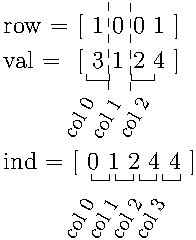
\includegraphics[width=100pt]{csc_detailed_example.pdf}
\caption{The internal arrays of a \code{CSC} matrix}\end{figure}

The values are stored column-wise in \code{row} and \code{val}: first the column \code{0}, than column \code{1} and finally column \code{2} (nothing for column \code{3}). \code{ind} gives the first indices for each column: \code{ind{[}0{]} == 0} gives the start of column \code{0},
\code{ind{[}1{]} == 1} gives the start of column \code{1}, etc. This means that \code{ind{[}j+1{]} - ind{[}j{]}} returns the number of elements in column \code{j}.


\subsection{How to run through a \texttt{CSC} matrix}
\label{sparse_matrix_formats:how-to-run-through-a-csc-matrix}
To find all triplets \((i, j, v)\):

\begin{Verbatim}[commandchars=\\\{\}]
\PYG{k}{for} \PYG{n}{j} \PYG{k+kn}{from} \PYG{l+m+mi}{0} \PYG{o}{\PYGZlt{}}\PYG{o}{=} \PYG{n}{j} \PYG{o}{\PYGZlt{}} \PYG{n}{ncol}\PYG{p}{:}
    \PYG{k}{for} \PYG{n}{k} \PYG{k+kn}{from} \PYG{n+nn}{ind}\PYG{p}{[}\PYG{n}{j}\PYG{p}{]} \PYG{o}{\PYGZlt{}}\PYG{o}{=} \PYG{n}{k} \PYG{o}{\PYGZlt{}} \PYG{n}{ind}\PYG{p}{[}\PYG{n}{j}\PYG{o}{+}\PYG{l+m+mi}{1}\PYG{p}{]}\PYG{p}{:}
        \PYG{n}{i} \PYG{o}{=} \PYG{n}{row}\PYG{p}{[}\PYG{n}{k}\PYG{p}{]}
        \PYG{n}{v} \PYG{o}{=} \PYG{n}{val}\PYG{p}{[}\PYG{n}{k}\PYG{p}{]}
\end{Verbatim}


\chapter{\textbf{\texttt{CySparse}}`s sparse matrix classes hierachy}
\label{sparse_mat_hierarchy:cysparse-s-sparse-matrix-classes-hierachy}\label{sparse_mat_hierarchy::doc}\label{sparse_mat_hierarchy:sparse-matrix-hierarchy}

\section{The hierarchy at a glance}
\label{sparse_mat_hierarchy:the-hierarchy-at-a-glance}

\section{The \texttt{SparseMatrix} class}
\label{sparse_mat_hierarchy:the-sparsematrix-class}

\section{The \texttt{MutableSparseMatrix} class}
\label{sparse_mat_hierarchy:the-mutablesparsematrix-class}

\section{The \texttt{ImmutableSparseMatrix} class}
\label{sparse_mat_hierarchy:the-immutablesparsematrix-class}

\chapter{Code generation}
\label{code_generation::doc}\label{code_generation:code-generation}

\section{\textbf{\texttt{generate\_code}} in more details}
\label{code_generation:generate-code-in-more-details}\label{code_generation:id1}
To generate the whole library:

\begin{Verbatim}[commandchars=\\\{\}]
python generate\PYGZus{}code.py \PYGZhy{}r cysparse
\end{Verbatim}

To generate a specific file, for instance the file \code{csr\_mat.cpd}:

\begin{Verbatim}[commandchars=\\\{\}]
python generate\PYGZus{}code.py \PYGZhy{}r cysparse \PYG{l+s+s1}{\PYGZsq{}csr\PYGZus{}mat.cpd\PYGZsq{}}
\end{Verbatim}

You can use


\chapter{\textbf{\texttt{CySparse}} for library maintainers}
\label{cysparse_lib_mainteners:cysparse-for-library-mainteners}\label{cysparse_lib_mainteners::doc}\label{cysparse_lib_mainteners:cysparse-for-library-maintainers}
\begin{notice}{warning}{Warning:}
TO REWRITE COMPLETELY
\end{notice}

The main difficulty to maintain the \textbf{\texttt{CySparse}} library is to understand and master the automatic code generation from templated source code. We use the template engine \textbf{\texttt{Jinja2}} and some hard coded
conventions. We explain and justify these conventions in the following sections.

The sparse matrix formats are detailed in the section {\hyperref[sparse_matrix_formats:sparse-matrix-formats]{\emph{\DUspan{}{Sparse Matrix Formats}}}}.


\section{Versions}
\label{cysparse_lib_mainteners:versions}
The version is stored in the file \code{\_\_init\_\_.py} of the \code{cysparse} subdirectory:

\begin{Verbatim}[commandchars=\\\{\}]
\PYG{n}{\PYGZus{}\PYGZus{}version\PYGZus{}\PYGZus{}} \PYG{o}{=} \PYG{l+s}{\PYGZdq{}}\PYG{l+s}{0.1.0}\PYG{l+s}{\PYGZdq{}}
\end{Verbatim}

The version can be anything inside the quotes but this line has to be on its own and start with \code{\_\_version\_\_ = "} (notice the one space before and after the equal sign). See the function \code{find\_version()} in the file \code{setup.cpy} for more details.


\section{Meta-programming aka code generation}
\label{cysparse_lib_mainteners:meta-programming-aka-code-generation}
\textbf{\texttt{CySparse}} allows the use of different types at run time and most typed classes comes in different typed flavours. This feature comes with a price. Because we wanted to write the library completely
in \textbf{\texttt{Cython}}, we decided to go for the explicit template route, i.e. we write \textbf{templated source code} and and use \textbf{explicit names} in the source code.
This automatic generation process ask for some rigour and takes some time to master. If you follow the next conventions stricly, you should be fine. If you don't follow them then probably the code won't even compile or
if it does you might generate difficult to find bugs. Trust me on this one.

\begin{notice}{warning}{Warning:}
Follow the conventions stricly to write templated source code.
\end{notice}


\subsection{Justifications}
\label{cysparse_lib_mainteners:justifications}
Following conventions is not always easy, especially if you don't understand them. In this sub-section we try to convince you or at least we try to explain and justify some choices I (Nikolaj) made (and try to follow).

These conventions were made with the following purpose in mind:
\begin{itemize}
\item {} 
respect the DRY (Don't Repear Yourself) principle;

\item {} 
if the conventions are not followed, the code shouldn't compile;

\item {} 
prefer static over dynamic dispatch;

\item {} 
use typed variables whenever possible;

\item {} 
keep the code simple whenever it doesn't sacrifice to efficiency even if the solutions are not Pythonesque;

\end{itemize}

We develop these key ideas in the following sub-sections.


\subsubsection{Respect the DRY principle}
\label{cysparse_lib_mainteners:respect-the-dry-principle}
Don't write the same code twice. This means of course than whenever you can factorize some common code, you should do so but in our case, because we lack the notion of \emph{templates} (like \textbf{\texttt{C++}} templates), we
\textbf{have} to repeat ourselves and rewrite the classes with different types. This is the main reason to use a template engine and templated code. That said, some code has been duplicated because I (Nikolaj) could not find
how to make it work in \textbf{\texttt{Cython}}. One example is the proxy classes: they all share common code. I wasn't able to make them inherit from a base class \footnote{
See \href{https://github.com/PythonOptimizers/cysparse/issues/113}{https://github.com/PythonOptimizers/cysparse/issues/113} for more about this issue.
}.


\subsubsection{If the conventions are not respected, the code shouldn't compile}
\label{cysparse_lib_mainteners:if-the-conventions-are-not-respected-the-code-shouldn-t-compile}
To enforce the use of the conventions, we try to enforce them by the compiler (whether the \textbf{\texttt{C}}, the \textbf{\texttt{Cython}} or \textbf{\texttt{Python}} compiler). Often, you'll find that templated code have guards to ensure that
types are recognized and otherwise to generate garbish that won't compile.

The name convention is written explicitely: if you don't respect it, you won't be able to use the \textbf{\texttt{generate\_code.py}} script. This is on purpose.


\subsubsection{Prefer static over dynamic dispatch}
\label{cysparse_lib_mainteners:prefer-static-over-dynamic-dispatch}
Even if \textbf{\texttt{Python}} is a dynamic language, efficient \textbf{\texttt{Cython}} code \textbf{needs} typing. This typing can be done dynamically with long and tedious \code{if/then} combinations or we can let the compiler
do the dispatch in our place at compile time whenever possible. This is the main reason why there are as many \code{LLSparseMatrixView} classes as there are \code{LLSparseMatrix} classes. Strictly speaking, we don't need
more \code{LLSparseMatrixView} classes than the number of index types but then you need to dynamically dispatch some operations like the creation of a corresponding {}`{}`


\subsubsection{Use typed variables whenever possible}
\label{cysparse_lib_mainteners:use-typed-variables-whenever-possible}
\textbf{\texttt{Cython}} really shines when it can deduce some static typing, especially in numeric loops. Therefor try to type variables \textbf{if} you know their type in advance \footnote{
Use your intelligence and knowledge of \textbf{\texttt{Cython}}. Know when it makes a difference to type a variable.
}.

Our hope is to keep a nice balance between the difficulty of coding and the easiness to maintain the code. When generating automatically code, these two don't necessarily go hand in hand.

If you find some code that doesn't follow these conventions, report it or even better change it!


\subsection{Types}
\label{cysparse_lib_mainteners:types}

\subsubsection{Basic types}
\label{cysparse_lib_mainteners:basic-types}
For different reasons \footnote{
we use \textbf{\texttt{C99}} for its superiority compared to \textbf{\texttt{ANSI C}} (\textbf{\texttt{C89}} or \textbf{\texttt{C90}} which is the same). Among others:
\begin{itemize}
\item {} 
the INFINITY and NAN macros;

\item {} 
its complex types;

\item {} 
inline functions;

\end{itemize}
} (???)

We use the following basic types:

\begin{tabulary}{\linewidth}{|L|L|}
\hline
\textsf{\relax 
\textbf{\texttt{CySparse}}
} & \textsf{\relax 
C99 types
}\\
\hline
\code{INT32\_t}
 & 
\code{int}
\\
\hline
\code{UINT32\_t}
 & 
\code{unsigned int}
\\
\hline
\code{INT64\_t}
 & 
\code{long}
\\
\hline
\code{UINT64\_t}
 & 
\code{unsigned long}
\\
\hline
\code{FLOAT32\_t}
 & 
\code{float}
\\
\hline
\code{FLOAT64\_t}
 & 
\code{double}
\\
\hline
\code{FLOAT128\_t}
 & 
\code{long double}
\\
\hline
\code{COMPLEX64\_t}
 & 
\code{float complex}
\\
\hline
\code{COMPLEX128\_t}
 & 
\code{double complex}
\\
\hline
\code{COMPLEX256\_t}
 & 
\code{long double complex}
\\
\hline\end{tabulary}



\subsubsection{Two categories of types}
\label{cysparse_lib_mainteners:two-categories-of-types}
We allow the use of different types at two levels:
\begin{itemize}
\item {} 
for the indices (\code{INT32\_t} and \code{INT64\_t}) \footnote{
We don't want to enter into the debate unsigned vs signed integers. Accept this as a fact. Beside, we use internally negative indices.
};

\item {} 
for the matrix elements (\textbf{all} the basic types).

\end{itemize}


\subsubsection{Add (or remove) a new type}
\label{cysparse_lib_mainteners:add-or-remove-a-new-type}

\subsection{Conventions}
\label{cysparse_lib_mainteners:conventions}

\subsubsection{File names and directories}
\label{cysparse_lib_mainteners:file-names-and-directories}
To keep the generation of code source files as simple as possible, we follow some conventions. This list of conventions is \textbf{strict}: if you depart from these conventions, the code will \textbf{not} compile.
\begin{itemize}
\item {} 
\textbf{Don't} use fused types: this feature is too \textbf{experimental}.

\item {} 
Template files have the following extensions:

\begin{tabulary}{\linewidth}{|L|L|L|}
\hline
\textsf{\relax 
\textbf{\texttt{Cython}}
} & \textsf{\relax 
\textbf{\texttt{CySparse}} template
} & \textsf{\relax 
File type
}\\
\hline
\code{.pxd}
 & 
\code{.cpd}
 & 
Definition files.
\\
\hline
\code{.pyx}
 & 
\code{.cpx}
 & 
Implementation files.
\\
\hline
\code{.pxi}
 & 
\code{.cpi}
 & 
Text files to insert verbatim.
\\
\hline\end{tabulary}


For python files:

\begin{tabulary}{\linewidth}{|L|L|L|}
\hline
\textsf{\relax 
\textbf{\texttt{Python}}
} & \textsf{\relax 
\textbf{\texttt{CySparse}} template
} & \textsf{\relax 
File type
}\\
\hline
\code{.py}
 & 
\code{.cpy}
 & 
Python module files.
\\
\hline\end{tabulary}


\item {} 
Any \emph{template} directory must \textbf{only} contain the template files and the generated files. This is because
all files with the right extension are considered as templates and all the other files are considered as generated
(and can be thus automatically erased). This clear distinction allows also to have a strict separation between
automatically generated files and the rest of the code.

\item {} 
Index types are replaced whenever the variable \code{@index@} is encountered, Element types are replaced whenever the variable \code{@type@} is encountered.

\item {} 
Generated \textbf{file names}:
\begin{itemize}
\item {} 
for a file \code{my\_file.cpx} where we only replace an index type \code{INT32\_t}: \code{my\_file\_INT32\_t.pyx};

\item {} 
for a file \code{my\_file.cpx} where we replace an index type \code{INT32\_t} \textbf{and} an elment type \code{FLOAT64\_t}: \code{my\_file\_INT32\_t\_FLOAT\_t.pyx}.

\end{itemize}

\item {} 
Generated \textbf{class/method/function names}:

\end{itemize}


\subsubsection{\textbf{\texttt{Jinja2}} conventions}
\label{cysparse_lib_mainteners:jinja2-conventions}

\subsection{Automatic generation scripts}
\label{cysparse_lib_mainteners:automatic-generation-scripts}
\textbf{All} generated files can be generated by invoking a \textbf{single} script:

\begin{Verbatim}[commandchars=\\\{\}]
python generate\PYGZus{}code.py
\end{Verbatim}


\section{Conventions}
\label{cysparse_lib_mainteners:id5}

\subsection{Names}
\label{cysparse_lib_mainteners:names}

\subsection{Types}
\label{cysparse_lib_mainteners:id6}
\textbf{All} classes are typed and \emph{almost} all algorithms used specialized typed variables. Many algorithm are specialized for \textbf{one} type of variable. This allows to have optimized algorithms but at the detriment of being able to mix types. For instance, most of the methods of sparse matrices only works for \textbf{one} \code{dtype} and \textbf{one} \code{itype}.


\subsection{How to expose \texttt{enum}s to \textbf{\texttt{Python}}}
\label{cysparse_lib_mainteners:how-to-expose-enums-to-python}
Even if recently \textbf{\texttt{Cyhton}} exposes automagically \code{enum}s to \textbf{\texttt{Python}} (see \href{https://groups.google.com/forum/\#!topic/cython-users/gn1p6znjoyE}{https://groups.google.com/forum/\#!topic/cython-users/gn1p6znjoyE}), don't count on it. The convention is
to expose equivalent strings to the user. This string is then translated internally by the corresponding \code{enum}. For instance, the \code{enum} value \code{UMFPACK\_A} \textbf{\texttt{UmfPack}} system parameter can be
given as the string \emph{`UMFPACK\_A'} by the user (as a parameter to a \emph{solve()} method for instance). Internally, this string is translated:

\begin{Verbatim}[commandchars=\\\{\}]
\PYG{k}{def} \PYG{n+nf}{solve}\PYG{p}{(}\PYG{o}{.}\PYG{o}{.}\PYG{o}{.}\PYG{p}{,} \PYG{n}{umfpack\PYGZus{}sys\PYGZus{}string}\PYG{o}{=}\PYG{l+s}{\PYGZsq{}}\PYG{l+s}{UMFPACK\PYGZus{}A}\PYG{l+s}{\PYGZsq{}}\PYG{p}{,} \PYG{o}{.}\PYG{o}{.}\PYG{o}{.}\PYG{p}{)}\PYG{p}{:}
    \PYG{n}{cdef}\PYG{p}{:}
        \PYG{n+nb}{int} \PYG{n}{umfpack\PYGZus{}sys} \PYG{o}{=} \PYG{n}{UMFPACK\PYGZus{}SYS\PYGZus{}DICT}\PYG{p}{[}\PYG{n}{umfpack\PYGZus{}sys\PYGZus{}string}\PYG{p}{]}
    \PYG{o}{.}\PYG{o}{.}\PYG{o}{.}
\end{Verbatim}

In \textbf{\texttt{Cython}} code, you are free to directly use the \code{enum} itself.


\section{Class hierarchy}
\label{cysparse_lib_mainteners:class-hierarchy}
The class hierarchy may seems strange at first and indeed is strange. In my wildest dreams (I = Nikolaj) I would like to have a base class \code{MatrixLike} from which all other classes inherit.
Something like this \footnote{
Note that some classes don't exist yet.
}:
\begin{figure}[htbp]
\centering
\capstart

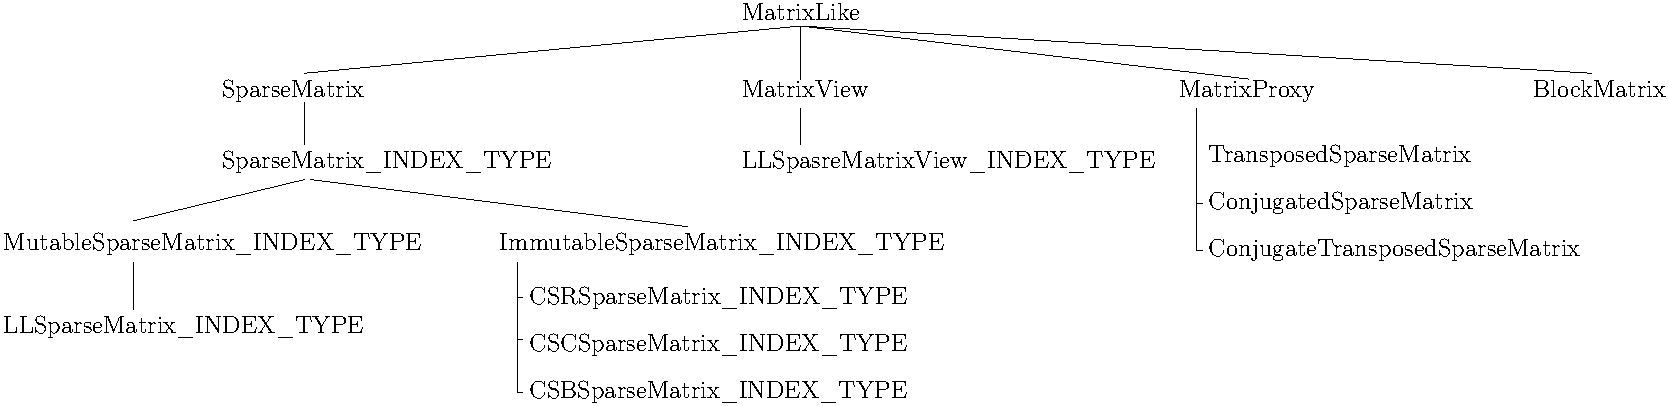
\includegraphics[width=600pt]{ideal_class_hierarchy.pdf}
\caption{The ideal (?) class hierarchy}\end{figure}

While this makes perfect sense at first, it is not very practical with the current situation of \textbf{\texttt{Cython}} and its inability to really use \emph{templates}. For instance, the \code{MatrixLike} class should have
\code{nrow} and \code{ncol} as attributes but this cannot be done for the moment as both attributes are better typed \footnote{
Of course, one could argue that we could use non typed attributes in \code{MatrixLike}.
}. Thus, \code{nrow} and \code{ncol} must be defined in \code{SparseMatrix\_INDEX\_TYPE}, and then
again in \code{LLSparseMatrixView\_INDEX\_TYPE} and then again... We could define a base \code{MatrixLike\_INDEX\_TYPE} class and so on.But the point is that \code{MatrixLike} would be quite empty. Basically, I tried to keep it simple and
without too many inheritance. The resulting class hierarchy is far from optimal (and \textbf{is} strange \footnote{
Especially with the \code{SparseMatrix} class split in two (\code{SparseMatrix} and \code{SparseMatrix\_INDEX\_TYPE})), \code{LLSparseMatrixView\_INDEX\_TYPE} on its own and
non typed proxies.
}) but is - in my view - a good compromise between code complexity (maintenance), code
duplication and ease of use but also Cython's limitations (See \footnotemark[1]).

The current situation is:
\begin{figure}[htbp]
\centering
\capstart

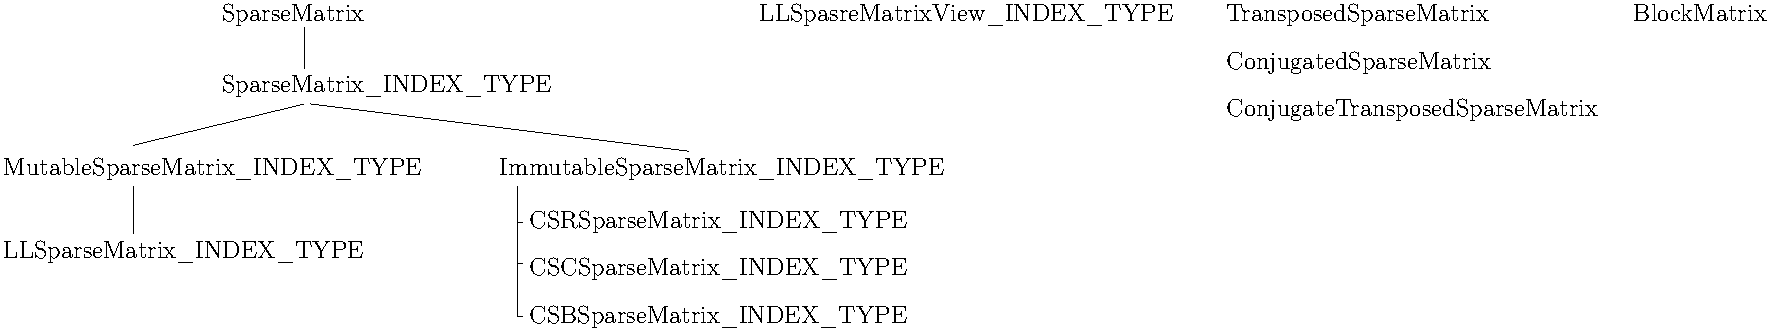
\includegraphics[width=700pt]{current_class_hierarchy.pdf}
\caption{Current class hierarchy}\end{figure}

which involves some code duplication and the use of global functions.


\chapter{Afterthougths}
\label{afterthougths::doc}\label{afterthougths:afterthougths}
This

Some pages of this documentation display equations via the \href{http://www.math.union.edu/~dpvc/jsMath/welcome.html}{jsMath} package. They should
look reasonably good with most setups but the best rendering is obtained by
installing the TeX fonts. Please refer to
\href{http://www.math.union.edu/~dpvc/jsMath/users/welcome.html}{http://www.math.union.edu/\textasciitilde{}dpvc/jsMath/users/welcome.html}.


\chapter{Indices and Tables}
\label{contents:indices-and-tables}\begin{itemize}
\item {} 
\DUspan{xref,std,std-ref}{genindex}

\item {} 
\DUspan{xref,std,std-ref}{modindex}

\item {} 
\DUspan{xref,std,std-ref}{search}

\end{itemize}



\renewcommand{\indexname}{Index}
\printindex
\end{document}
